\section{Flexible Resource Allocation Mechanisms}
\label{sec:flexible-resource-allocation-mechanisms}
As explained in the last Section, all previous research outlined in Section~\ref{sec:related-work} is incompatible
with our resource elastic optimisation problem in Section~\ref{sec:problem-formulation}. Therefore in this
section, we propose three mechanisms for solving this optimisation problem: an approximation algorithm and two
auction-based mechanisms.

The optimisation problem is a extended version of the knapsack problem, which is often solved using an dynamic
programming method that has pseudo-polynomial time complexity~\cite{}. The solution requires building a table of items to bags
allocation. For our problem, as the resource speeds must be considered at the same time, such a solver can are
infeasible due to both the space and time complexity required.

Because of this issue of allocating both tasks to a server and a server's resources to a task, this work proposes an
approximation algorithm where tasks are allocated to a server with resources in series not in parallel. The centralised
greedy algorithm (detailed in Subsection~\ref{subsec:greedy-algorithm}) ranks tasks that are each allocated to a server
with resources with each stage using an separate ranking function. This algorithm has a social welfare lower bound
of $\frac{1}{\left|J\right|}$, however in practice achieves close to the theoretical optimal while running with
polynomial time complexity.

As task users can be self-interested, they may report their task values or requirements strategically. Traditionally,
VCG~\cite{vickrey,Clarke,groves} is used for such systems due to its ability to use any optimisation problem to
calculate a task price. However, due to the difficulty of calculating the optimal allocation for this problem, VCG is
infeasible to use in this application. Therefore, to deal with self-interested users, we propose two auction-based
mechanisms. The first being an incentive-compatible auction using the centralised greedy algorithm
(Section~\ref{subsec:critical-value-auction}) and the second being a novel Decentralized Iterative
Auction (Section~\ref{subsec:decentralised-iterative-auction}) that does not require users to reveal the task value.

\subsection{Greedy Algorithm}
\label{subsec:greedy-algorithm}
To solve a knapsack problem, a greedy approximation algorithm is often used~\cite{}. We have applied a similar approach
to this problem specified in subsection~\ref{subsec:optimisation-problem}. As a result of the elastic nature of task
resources, an additional stage is required once a task has been allocated to a server in order to determine the task's
resource speeds.

\begin{wrapfigure}{r}{0.5\linewidth}
    \centering
    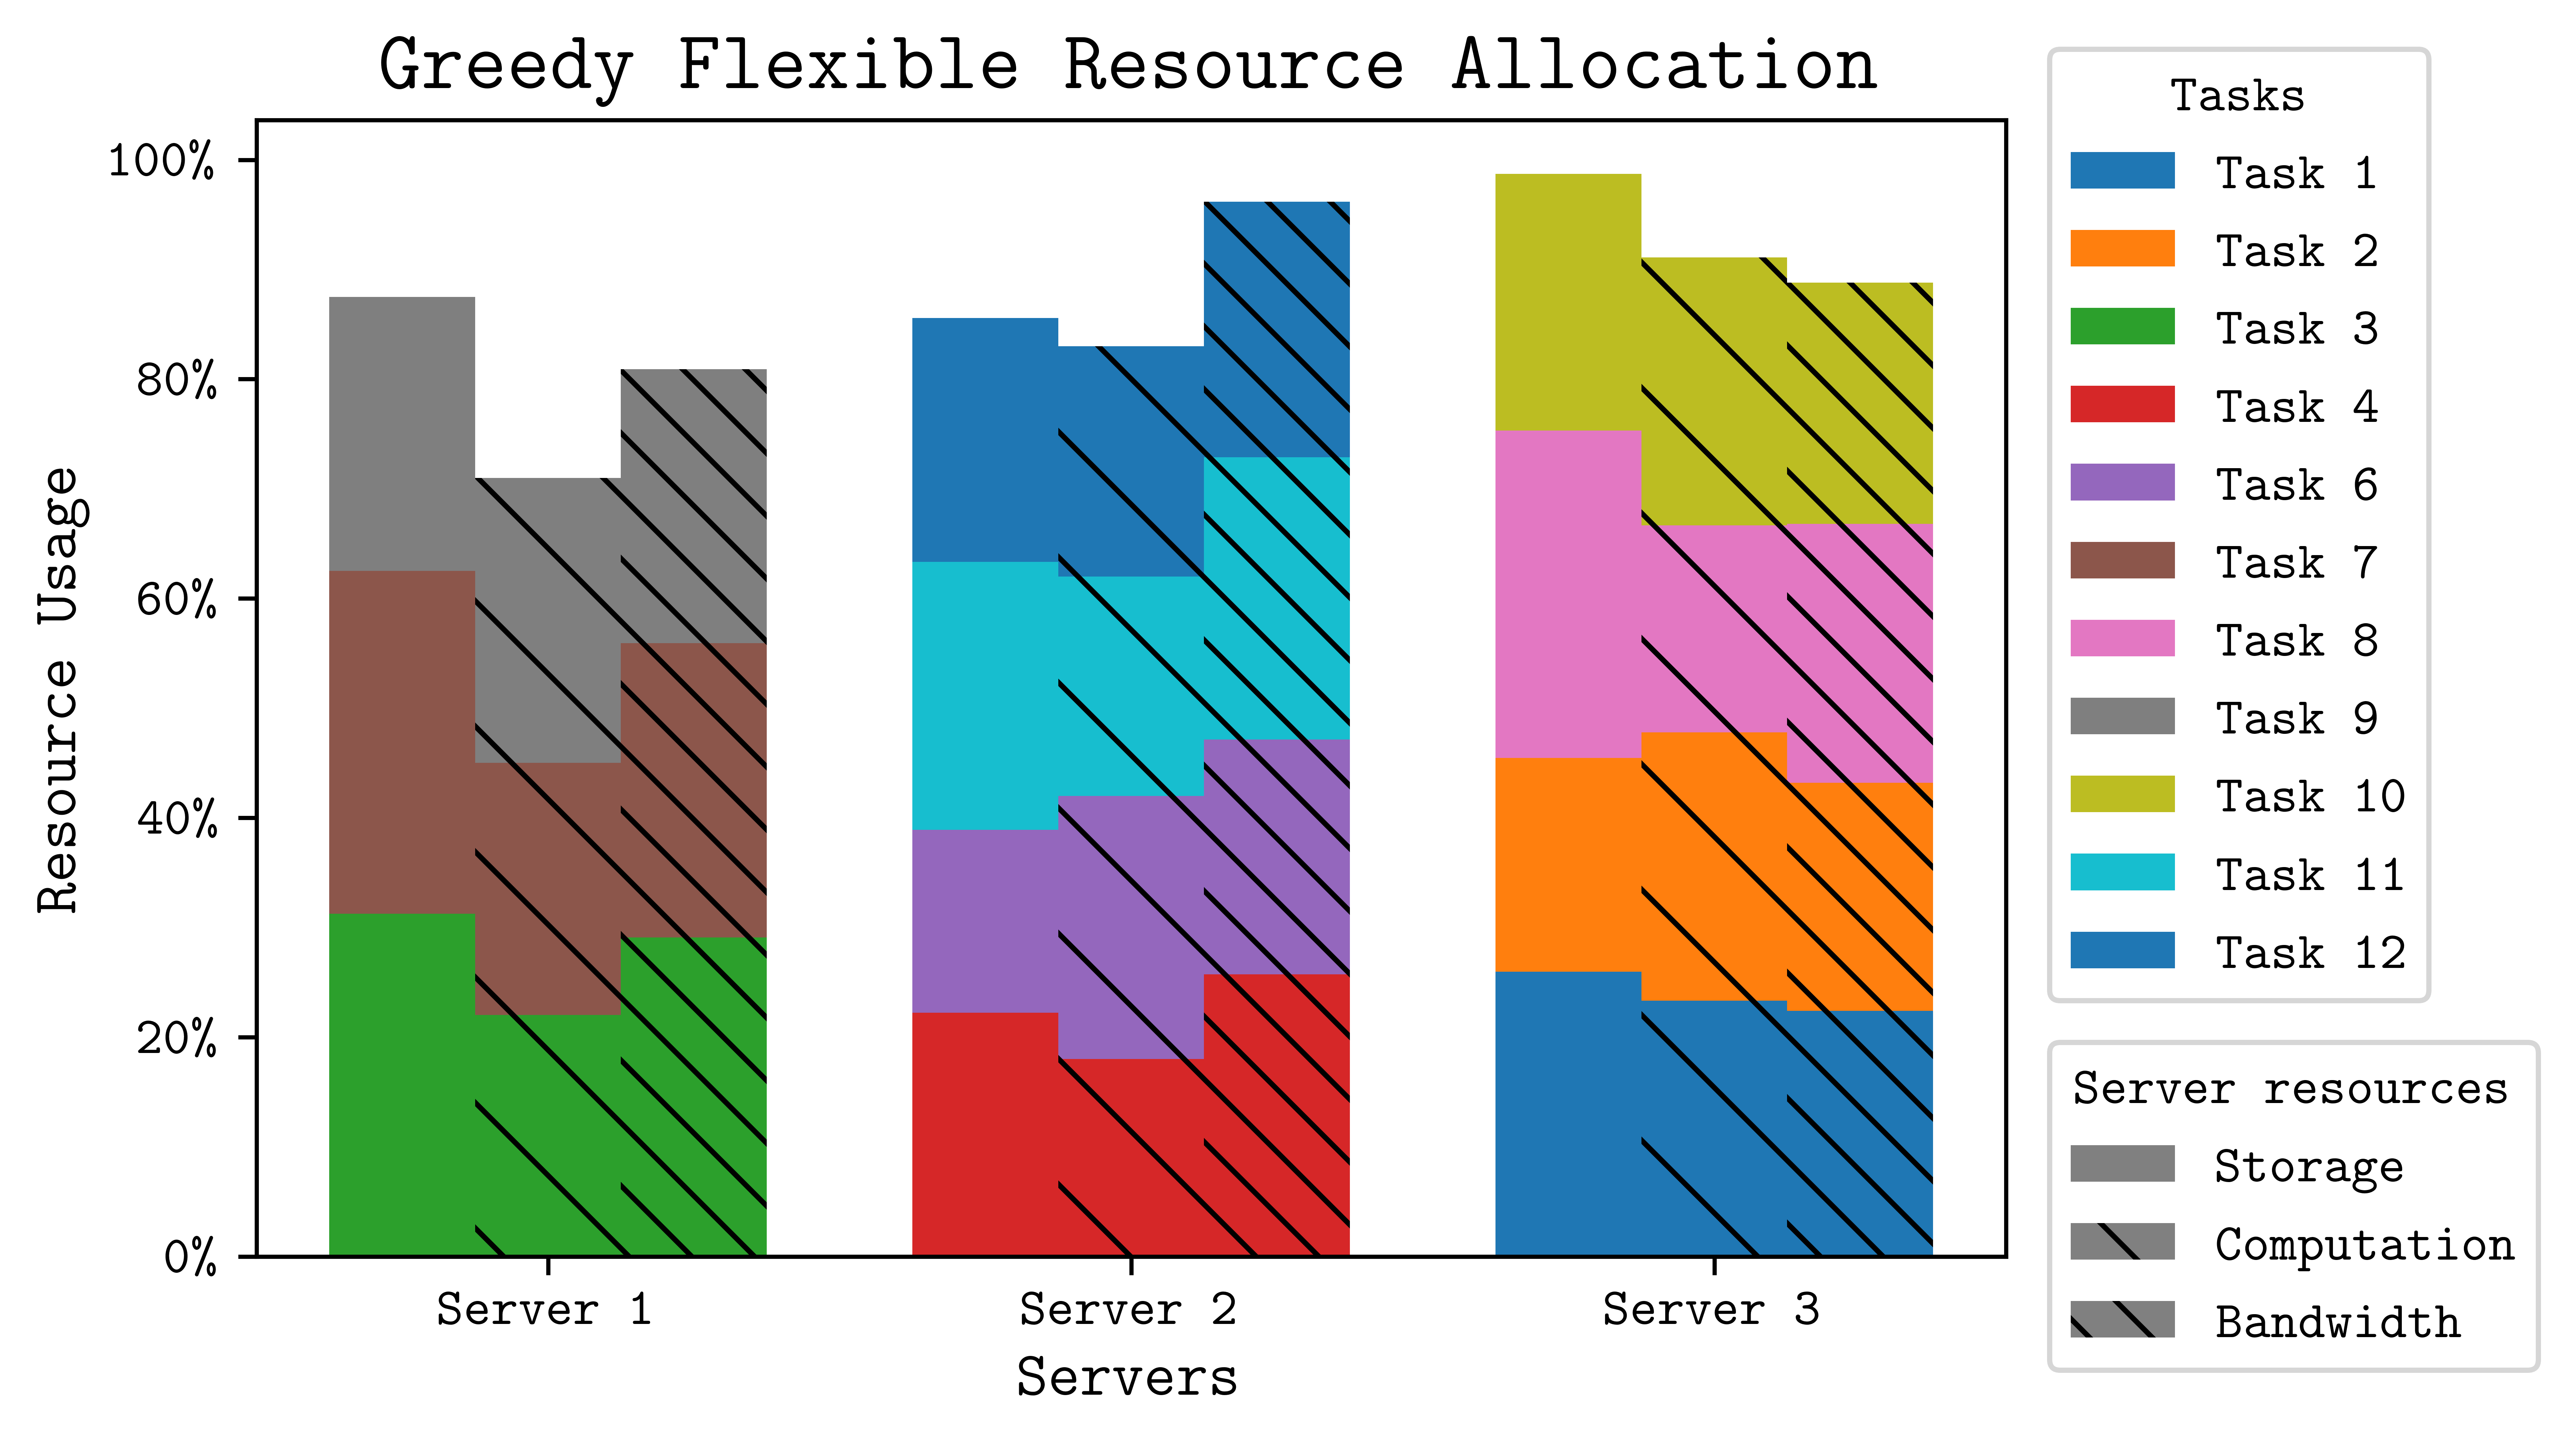
\includegraphics[width=\linewidth]{figs/allocation/greedy_flexible_resource_allocation.png}
    \caption{Example Greedy allocation using the model from table~\ref{tab:example-tasks-properties}
    and~\ref{tab:example-servers-properties}}
    \label{fig:example-greedy-allocation}
\end{wrapfigure}

More specifically, the greedy algorithm has two stages; stage one sorts the list of tasks based on the value
density of each task calculated using task attributes: value, required resources and deadline. The second
stage uses the sorted list of tasks to iterate through applying two heuristics to select the server based on
available server resources and to allocate resources based on the available server resources and the required resources
of the task.

Using the example case from subsection~\ref{subsec:example-problem-case}, the greedy algorithm can complete 11/12 of
the tasks achieving XX\% more social welfare than the fixed solution. This is due to the algorithm being unable to % TODO
consider other tasks resource requirement while allocating resource. The greedy algorithm used for the value density
function, $\frac{v_j \cdot d_j}{s_j + w_j + r_j}$, for server selection, $\text{argmin}_{\forall i \in I} S^{'}_i \cdot W^{'}_i \cdot R^{'}_i$
for task $j$ and servers $I$ and for the resource allocation is
$\text{argmin}_{s^{'}_j, w^{'}_j, r^{'}_j} \left(\frac{w^{'}_j}{W^{'}_i}\right)^3 + \left(\frac{s^{'}_j + r^{'}_j}{R^{'}_i}\right)^3$
is task $j$ and server $i$.

\begin{algorithm}
    \caption{Pseudo code of Greedy Algorithm}
    \label{alg:greedy-mechanism}
    \begin{algorithmic}
        \REQUIRE $J$ is the set of tasks and $I$ is the set of servers
        \REQUIRE $S^{'}_i$, $W^{'}_i$ and $R^{'}_i$ is the available resources
            (storage, computation and bandwidth respectively) of server $i$
        \REQUIRE $v(j)$ is the value density function of task $j$
        \REQUIRE $s(j, I)$ is the server selection function of task $j$ and set of servers $I$ returning the best
            server, or $\emptyset$ if the task is not able to be run on any server
        \REQUIRE $r(j, i)$ is the resource allocation function of a task and server returning the
            loading, compute and sending speeds
        \REQUIRE $\text{sort}(X, f)$ is a function that returns a sorted list of elements in descending order, based
            on a set of elements $X$ and a function for comparing elements $f$

        \STATE{$J^{'} \leftarrow sort(J, v)$}
        \FORALL{$j \in J^{'}$}
            \STATE{$i \leftarrow s(j, I)$}
            \IF{$i \neq \emptyset$}
                \STATE{$s^{'}_j, w^{'}_j, r^{'}_j \leftarrow \gamma(j, i)$}
                \STATE{$x_{i,j} \leftarrow 1$}
            \ENDIF
        \ENDFOR
    \end{algorithmic}
\end{algorithm}

\subsubsection{Greedy Lower Bound}
\label{subsubsec:greedy-lower-bound}
The lower bound of the algorithm is $\frac{1}{\left|J\right|}$ (where $\left|J\right|$ is the number of tasks) with
the task value as the value density function. This lower bound is not affected by the server selection policy or the
resource allocation policy. \\
However in testing, we found that the task value function is not the best value density heuristic as it does not
consider the effect of deadlines or the required resources of the task. In Section~\ref{sec:empirical-results}, we
considered a wide range of heuristics, showing the results of the best heuristics over a range of settings.

\begin{theorem}
    The lower bound of the greedy mechanism is $\frac{1}{n}$ of the optimal social welfare.
\end{theorem}
\begin{proof}
    Due to a task not considering other task's resource requirements then no matter the server selection or resource
    allocation function, it can't be guaranteed that subsequent tasks can be allocated to any server. As a result,
    the algorithm can be guaranteed to achieve at least $\frac{1}{n}$ of the optimal social welfare by using a
    value density function ($v(j) = j_v$). Using this, the first task from the sorted task list will have the maximum task
    value meaning the lower bound of the algorithm is $\frac{1}{n}$ of the optimal social welfare.
\end{proof}

\subsubsection{Greedy Time Complexity}
\label{subsubsec:greedy-time-complexity}
Using the greedy mechanism (algorithm~\ref{alg:greedy-mechanism}), the time complexity is polynomial,
$O(\left|J\right| \left|I\right|)$.
\begin{theorem}
    Time complexity of the greedy mechanism is $O(\left|J\right| \left|I\right|)$, where $\left|J\right|$ is the number
    of tasks and $\left|I\right|$ is the number of servers. Assuming that the value density and resource allocation
    heuristics have constant time complexity and the server selection function is $O(\left|I\right|)$.
    %% TODO to check if the resource allocation heuristic is constant time complexity (KKT) probably wrong
\end{theorem}
\begin{proof}
    The time complexity of stage 1 of the mechanism is $O(\left|J\right| \log(\left|J\right|))$ due to sorting the
    tasks and stage 2 has complexity $O(\left|J\right| \left|I\right|)$ due to looping over all the tasks and
    applying the server selection and resource allocation heuristics. Therefore the overall time complexity is
    $O(\left|J\right| \left|I\right| + \left|J\right| \log(\left|J\right|) = O(\left|J\right| \left|I\right|)$.
\end{proof}

\subsection{Critical Value Auction}
\label{subsec:critical-value-auction}
Due to the problem case being non-cooperative, if the greedy mechanism was used to allocate resources such that the
value is the price paid. This would be open to manipulation and misreporting of task attributes like the value,
deadline or resource requirements. Therefore, in this section we propose an auction that is strategy-proof
(weakly dominant incentive compatible) so users have no incentive to misreport task attributes.

Single-Parameter domain auctions are extensively studied in mechanism design~\cite{nisan2007algorithmic_228} and are
used where an agent's valuation function can be represented as a single value. The task price is calculated by finding
the critical value, the minimum task price required for the task still allocated to any server. This has
been shown to be a strategy-proof~\cite{nisan2007algorithmic_229_230} auction making it a weakly dominant strategy for
a user to honestly reveal a task's attribute.

The auction is implemented using the greedy mechanism from section~\ref{subsec:greedy-algorithm} by finding an initial
allocation using every task's reported value. Then for each task that is allocated, the task price is equal to the
critical value is found by finding the minimum value of the task such that it is still allocated. \\
To find the minimum value is a two-step process of removing the task from the list of tasks then running the greedy
mechanism however after each task is allocated. Then a check is done if the critical task could be allocated to any
server. This is a constant time complexity operation by assuming that the server would allocate all of its available
resources for the deadline constant (eq~\ref{eq:task-deadline}). If the task can't be allocated to any server then the
value density of last task allocated is equalled to the required value density of the critical task (this assumes that
in the sorted list, the critical task would appear ahead thus a minor amount could be add thus to guarantee the
critical task is above). Using the value density and the value density function, through finding the inverse of the
value density function, with regards to the task value allows the task critical value to be calculated.

\subsubsection{Critical Value Auction Time Complexity}
\label{subsubsec:critical-value-auction-time-complexity}
The time complexity of the auction is $O(\left|J\right| \left|J\right| \left|I\right|)$, the greedy
mechanism repeated $\left|J\right|$ due to calculating each task's critical value.
\begin{theorem}
    The time complexity of the critical value auction is $O(\left|J\right| \left|J\right| \left|I\right|)$.
\end{theorem}
\begin{proof}
    %% Todo to rewrite after algorithm made
    The auction uses the greedy algorithm (subsection~\ref{subsec:greedy-algorithm}), that has time complexity of
    $O(\left|J\right| \left|I\right|)$. For each task allocated by the greedy algorithm, the critical value must be
    found. To find the critical value of each task requires rerunning a modified greedy algorithm, such that after each
    task is allocated a check is done to see if the current task could be allocated to any server. This is done by repeating the server selection and resource allocation functions for each task (excluding
    the critical task) with time complexity,
    $O(\left|J\right| \left|I\right|)$, until the critical task can no longer be allocated to any server (a constant time function).
    The task's critical value is calculated in constant time function. As a result, the time complexity for
    calculating the critical value for an individual task is $O(\left|J\right| \left|I\right|)$. Thus, the overall time
    complexity is $O(\left|J\right| \left|J\right| \left|I\right|)$ due to the critical value being
    found for every task.
\end{proof}

\subsubsection{Demonstrating that the Critical Value Auction is Strategyproof}
\label{subsubsec:critical-value-auction-strategyproof}
In order that the auction is strategyproof, the value density function must be
monotonic~\cite{nisan2007algorithmic_229_230}. This ensures that if a task misreports any attributes, it will result
in the value density of the task decreasing. Therefore a value density function must be in the form of
$\frac{v_j \cdot d_j}{\alpha(s_j, w_j, r_j)}$ such it is monotonic decreasing.
\begin{theorem}
    The value density function $\frac{v_j \cdot d_j}{\alpha(s_j, w_j, r_j)}$ is monotonic increasing for task $j$ assuming
    the function $\alpha(s_j, w_j, r_j)$ is monotonic increasing for each variable.
\end{theorem}
\begin{proof}
    In order to misreport the task value and deadline, misreported values must be less than their true value. Therefore
    if the value or deadline are decreased then the value density will likewise decrease. \\
    The opposite is true for a task's required resources (storage, compute and result data), as the misreported value
    must be greater than the true value otherwise the task would not be able to be completed. Therefore as the $\alpha$
    function is will increase as the resource requirements increase, the resulting value density will decrease. \\
    So in any case, the overall value density will decrease if the owner doesn't accurately report a task's attribute,
    resulting in the task paying more.
\end{proof}

\subsection{Decentralised Iterative Auction}
\label{subsec:decentralised-iterative-auction}
In some applications of edge cloud computing, keeping the value of a task a secret is important for example in
military-tactical networks. Therefore we propose a novel decentralised iterative auction based on the pricing principle
of the VCG auction~\cite{vickrey,Clarke,groves}. VCG auction calculates the price of an item by finding the
difference in social welfare if the item exists and does not exist.

Our proposed novel auction uses the same principle, except in reverse by finding the difference between the current
server revenue and the revenue when the task is required to be allocated with a price of zero. To cause the overall
revenue and servers revenue to increase, a small value called the Price change variable is added to the task price.

Our auction uses this principle by iteratively letting a task advertise its requirements to all the servers, who
respond with their price to run the task. This price is equal to the server's current revenue minus the solution to the
problem in subsection~\ref{subsubsec:decentralised-iterative-problem} plus a small value referred to as the price change
variable. This is done to ensure that the total server revenue increases by accepting the task. Once all of the servers
have responded, the task can compare the minimum server prices to its private evaluation. This allows the task to
privately select the server that it runs on (assumed to be the server with the lowest price) otherwise the task will
stop advertising as it knows that its evaluation is lower than the price of any server.

The algorithm~\ref{alg:dia} is a centralised version of the auction. It works through iteratively checking a currently
unallocated task to find the price if the task was currently allocated on a server. This is done through first solving
the program in section~\ref{subsubsec:decentralised-iterative-problem} which calculates the new revenue if the task was
forced to be allocated with a price of zero. The task price is equal to the current server revenue minus the new
revenue with the task allocated plus a price change variable in order to increase the revenue of the server. The
minimum price returned by $P(i, k)$ is then compared to the task's maximum reserve price (that would be private in the
equivalent decentralised algorithm) to confirm if the task is willing to pay at that price. If the task is willing then
the task is allocated to the minimum price server and the task price set to the agreed price. However in the process of
allocating a task then the currently allocated tasks on the server could be unallocated so these tasks allocation's and
price's are reset then appended to the set of unallocated tasks.

%% TODO recode the DIA
\begin{algorithm}
    \caption{Decentralised Iterative Auction}
    \label{alg:dia}
    \begin{algorithmic}
        \REQUIRE $I$ is the set of servers
        \REQUIRE $J$ is the set of unallocated tasks, that is initial the set of all tasks
        \REQUIRE $P(i, k)$ is the solution to the problem in section~\ref{subsubsec:decentralised-iterative-problem}
            using the server $i$ and new task $k$. The server's current tasks is known to itself and its current
            revenue from tasks so not passed as arguments.
        \REQUIRE $\leftarrow_R$ will randomly select an element from a set

        \WHILE{$|J| > 0$}
            \STATE{$j \leftarrow_R J$}
            \STATE{$p, i \leftarrow \min_{i \in I} P(i, j)$}
            \IF{$p \leq v_j$}
                \STATE{$p_j \leftarrow p$}
                \STATE{$x_{i, j} \leftarrow 1$}
            \ENDIF
            \STATE{$J \leftarrow J \setminus \{j\}$}
        \ENDWHILE
    \end{algorithmic}
\end{algorithm}

\subsubsection{Server revenue optimisation problem}
\label{subsubsec:decentralised-iterative-problem}
To find the optimal revenue for a server $m$ given a new task $n^{'}$ and a set of currently allocated tasks $N$ has a
similar formulation to the optimisation problem in section~\ref{subsec:optimisation-problem}. Except with an additional
variable for the task price $p_n$ for each task $n$.

\begin{align}
    \max & \sum_{\forall n \in N} p_n x_n\label{eq:dia-objective}\\
    \mbox{s.t.} \nonumber \\
    & \sum_{\forall n \in N} s_n x_n + s_{n^{'}} \leq S_m,\label{eq:dia-server-storage-constraint}\\
    & \sum_{\forall n \in N} w^{'}_n x_n + w_{n^{'}} \leq W_m, \label{eq:dia-server-computation-constraint}\\
    & \sum_{\forall n \in N} (r^{'}_n + s^{'}_n) \cdot x_n + (r^{'}_{n^{'}} + s^{'}_{n^{'}}) \leq R_m, \label{eq:dia-server-communication-constraint}\\
    & \frac{s_n}{s^{'}_n} + \frac{w_n}{w^{'}_n} + \frac{r_n}{r^{'}_n} \leq d_n, &~ \forall n \in N \cup \{n^{'}\} \label{eq:dia-task-deadline}\\
    & 0 < s^{'}_n < \infty, &~ \forall{n \in N \cup \{n^{'}\}} \label{eq:dia-loading-speeds}\\
    & 0 < w^{'}_n < \infty, &~ \forall{n \in N \cup \{n^{'}\}} \label{eq:dia-compute-speeds}\\
    & 0 < r^{'}_n < \infty, &~ \forall{n \in N \cup \{n^{'}\}} \label{eq:dia-sending-speeds}\\
    & x_n \in \{0,1\} &~ \forall{n \in N} \label{eq:dia-task-allocation}
\end{align}

The objective (Eq.~\eqref{eq:dia-objective}) is to maximize the price of all currently allocated tasks (not including
the new task as the price is zero). The server resource capacity constraints
(Eqs.~\eqref{eq:dia-server-storage-constraint},~\eqref{eq:dia-server-computation-constraint}
and~\eqref{eq:dia-server-communication-constraint}) are similar to the constraints in the standard model set out in
section~\ref{subsec:optimisation-problem} except with the assumption that the task $n^{'}$ is running so there is no
need to consider if it is running or not. The deadline and non-negative resource speeds constraints
(\ref{eq:dia-task-deadline},~\ref{eq:dia-loading-speeds},~\ref{eq:dia-compute-speeds} and~\ref{eq:dia-sending-speeds})
are all the same equation as the standard formulation for all the tasks plus the new task. As this formulation only
considers a single server, the task allocation constraint is not considered

\subsubsection{Decentralised Iterative Auction properties}
\label{subsubsec:decentralised-iterative-auction-properties}
For our proposed auction, we consider four important properties in auction theory.
\begin{itemize}
    \item Budget balanced - True. Since the auction can run without an auctioneer, the auction can be run in a
        decentralised system resulting in no ''middlemen'' taking some money meaning that all revenue goes straight to
        the servers from the tasks.
    \item Individually Rational - True. As the server need to confirm with the task if it is willing to pay an amount
        to be allocated, the task can check this against its secret reserved price preventing the task from ever paying
        more than it is willing.
    \item Incentive Compatible - False. While a task's cannot determine the choices of other task for which server they
        will choose, the order task pricing as this is random or lie about the task value as this information isn't
        revealed. Task's can misreport it's attributes to force other task's to make decisions that would otherwise
        result in the misreporting task from being deallocated from a server. For example, if task misreports some
        attributes it may result in it being cheaper for another task to select a different server. This would mean
        that misreported task from not being deallocated. However for large scale systems, intentionally misreporting
        such attribute is extremely difficult to profit from. This is empirically shown in
        subsection~\ref{subsec:possibility-of-misreporting-task-attributes-in-decentarlised-iterative-auction}.
    \item Economic efficiency - False. The allocation of task's to server is completely random until server becomes full,
        because of this initial allocation and the random selection of task's meaning that often task's result in a
        local maxima rather than the global maxima. As a result, the auction is not 100\% economically efficient
        however the local optima are often close to the global maxima as shown in
        subsection~\ref{subsec:evaluation-of-the-auction-mechanisms}.
\end{itemize}

While the auction is not incentive compatible and that task's do not pay the critical value unlike the critical value
auction, task's do pay the minimal amount for the task to be allocated. This is different from the critical value due
to the requirement that the value is found through a deterministic process, however as this auction randomly selects
task's from the set of unallocated tasks to find a task it can't be the task's critical value.

\subsection{Attributes of the proposed algorithms}
\label{subsec:attributes-of-proposed-algorithms}
In this paper, we have presented three mechanisms to solve the optimisation problem proposed in
section~\ref{subsec:optimisation-problem}. Table~\ref{tab:attributes_algorithms} considers a range of
important attributes of the proposed algorithm to allow easy comparison between the Greedy mechanism,
Critical Value auction and Decentralised Iterative auction.

\begin{table}[H]
    \begin{tabular}{|p{3cm}|c|c|c|}
        \hline
        \textbf{Attribute} & Greedy Algorithm & Critical Value Auction & Decentralised Iterative Auction \\ \hline
        Truthfulness & & Yes & No \\ \hline
        Optimality & No  & No & No \\ \hline
        Scalability & Yes & Yes & No \\ \hline
        Task information requirements from users & All & All & All except the task value \\ \hline
        Communication over heads & Low & Low & High \\ \hline
        Decentralisation & No  & No  & Yes \\ \hline
    \end{tabular}
    \caption{Attributes of the proposed algorithms: Greedy mechanism, Critical Value auction and
    Decentralised Iterative auction}
    \label{tab:attributes_algorithms}
\end{table}
